%=====================================================================
\section{Trees}
%=====================================================================

\begin{frame}
	\frametitle{Outline}
	
	\begin{itemize}
		\item Decision Trees
		\item Random Forests
		\item Gradient Boosted Trees
	\end{itemize}
\end{frame}

%=====================================================================
\subsection{Decision Trees}
%=====================================================================

\begin{frame}
	\frametitle{Decision Trees}
	\begin{columns}[onlytextwidth]
		\column{0.5\textwidth}
		\begin{itemize}
			\item Simple		
			\item Easy to interpret
			\item Decision trees are like wolves:
			
			Weak alone, strong together
			\item Around since 1984 
			
			(Breiman, Friedman)
		\end{itemize}
		
		\column{0.5\textwidth}
		\begin{figure}
			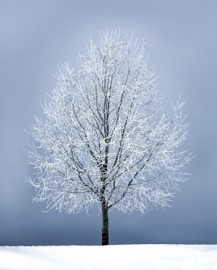
\includegraphics[width=0.7\textwidth]{pics/real_tree.jpg}
			\tiny{https://images.pexels.com/photos/3732527/pexels-photo-3732527.jpeg}
		\end{figure}
	\end{columns}
\end{frame}


\begin{frame}
	\frametitle{What is a Decision Tree?}
	\begin{columns}[onlytextwidth]
		\column{0.5\textwidth}
		\begin{block}{Greedy recursive partitioning}
			\begin{enumerate}
				\item Split: find best ``yes/no'' question on best feature to make total loss smaller
				\item Apply Step 1 recursively
			\end{enumerate}
		\end{block}
		
		\begin{block}{Predictions}
			\begin{itemize}
				\item Follow splits and use leaf value $\gamma_j$
				\item Usually, $\gamma_j$ is average response in leaf $j$
				\item Terminal regions $R_1, \dots, R_J$
				\item $\bx$ falls in leaf $j$ $\Leftrightarrow$ $\bx \in R_j$
				\item $\hat f(\bx) = \sum_{j = 1}^{J} \gamma_j \boldsymbol 1\{\bx \in R_j\}$
			\end{itemize}
		\end{block}
		
		\column{0.45\textwidth}
		\begin{figure}
			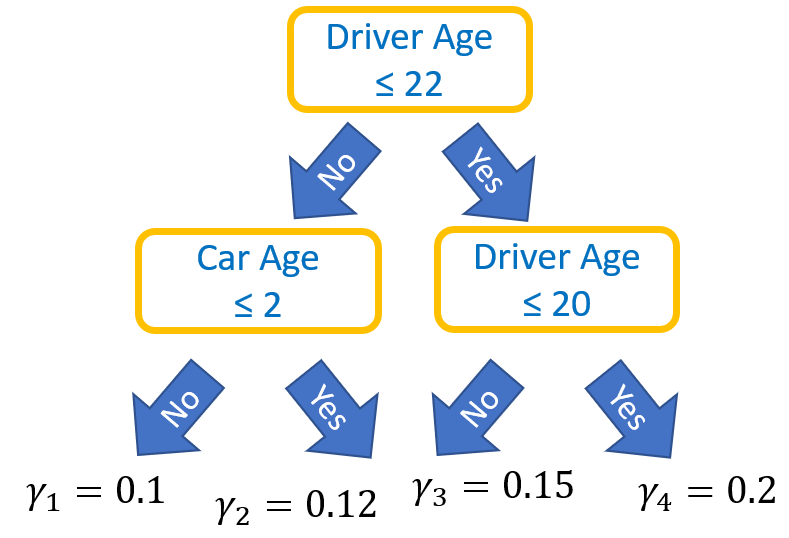
\includegraphics[width=1\textwidth]{../figs/a_tree.png}
		\end{figure}
		\centering The tree does a headstand
		
		\begin{example}
		\end{example}
	\end{columns}
\end{frame}

\begin{frame}
	\frametitle{Properties of Decision Trees}
	
	\begin{columns}[onlytextwidth]
		\column{0.5\textwidth}
		\begin{itemize}
			\item Outliers
			\item Missing values
			\item Categorical covariates
			\item Greedy
		\end{itemize}
		
		\column{0.5\textwidth}	
		\begin{itemize}
			\item Interactions
			\item Extrapolation
			\item Instability
			
			\vphantom{T}
		\end{itemize}
	\end{columns}
	
	\vfill 
	
	Most properties are inherited to groups/ensembles of decision trees
	
	\vfill
	
	From nearest neighbors to decision trees: Short video by Jerome Friedman: \url{https://www.youtube.com/watch?v=8hupHmBVvb0}
\end{frame}

%=====================================================================
\subsection{Random Forests}
%=====================================================================

\begin{frame}
	\frametitle{Random Forests}
	\begin{columns}[onlytextwidth]
		\column{0.5\textwidth}
		\begin{itemize}
			\item Combine many decision trees
			\item Perform very well
			\item Black Box
			\item Around since 2001 (Breiman)
			\item Why is combination of trees better than a single one?
		\end{itemize}
		
		\column{0.5\textwidth}
		\begin{figure}
			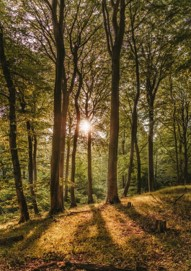
\includegraphics[width=0.6\textwidth]{pics/real_forest.jpg}
			\tiny{https://images.pexels.com/photos/1459534/pexels-photo-1459534.jpeg}
		\end{figure}
	\end{columns}
\end{frame}

\begin{frame}
	\frametitle{Ensembling and Bagging}
	\begin{block}{Ensembling}
		\begin{itemize}
			\item Combine multiple models (\alert{base learners}) to single one
			\item Example: $k$-nearest-neighbor with different $k$
			\item Often out-of-sample performance gain due to lower variance 
			
			$\rightarrow$ diversified stock portfolio
		\end{itemize}
	\end{block}
	
	\begin{block}{Algorithm: Bagging (\alert{B}ootstrap \alert{agg}regat\alert{ing})}
		\begin{enumerate}
			\item Select $B$ bootstrapped training data sets from the original training data
			\item Fit model $\hat f^{*j}(\bx)$ on each of them
			\item Return the bagged model 
			$
			\hat f(\bx) = \frac{1}{B} \sum_{j = 1}^B f^{*j}(\bx)
			$
		\end{enumerate}
	\end{block}
	
	\begin{example}
	\end{example}
\end{frame}

\begin{frame}
	\frametitle{Remarks on Bagging}
	
	\begin{itemize}
		\item Base learners
		\item Out-of-bag (OOB)
		\item Parallel computing
		\item Performance versus complexity
	\end{itemize}
\end{frame}

\begin{frame}
	\frametitle{From Bagging to Random Forests}
	A random forest is a bagged decision tree with an extra twist
	
	\begin{block}{Twist}
		\begin{itemize}
			\item Additional source of randomness
			\item Each split considers only random feature subset (often $p/3$ or $\sqrt p$)
			\item Additional decorrelation $\rightarrow$ stronger diversification
		\end{itemize}
	\end{block}
	
	\begin{block}{Algorithm: Random forest (regression)}
		\begin{enumerate}
			\item Select $B$ bootstrapped training data sets from the original training data
			\item Fit (usually deep) decision tree $\hat f^{*j}(\bx)$ on each of them. For each split, consider only random feature subset
			\item Return the random forest
			$
			\hat f(\bx) = \frac{1}{B} \sum_{j = 1}^B f^{*j}(\bx)
			$
		\end{enumerate}
	\end{block}
\end{frame}

\begin{frame}
	\frametitle{Comments on Random Forests}
	
	\begin{itemize}
		\item Number of trees
		\item Deep trees and diversification 
		\item Don't trust performance on the training set
		\item Parameter tuning
	\end{itemize}
	
	\vfill
	
	Regarding \alert{parameter tuning}: Short video by Adele Cutler on working with Leo Breiman: \url{https://www.youtube.com/watch?v=t8ooi_tJHSE}
	
	\vfill
	
	\begin{example}
	\end{example}
\end{frame}

\begin{frame}
	\frametitle{Interpreting a Black Box}
	\begin{columns}
		\column{0.3\textwidth}
		\begin{block}{Study for each model}
			\begin{enumerate}
				\item Performance
				\item Variable importance
				\item Effects
			\end{enumerate}
		\end{block}
		\column{0.7\textwidth}
		\begin{block}{XAI}
			\begin{itemize}
				\item e{\bf X}plainable {\bf A}rtificial {\bf I}ntelligence
				\item Collection of methods to interpret models
				\item Examples: Split-gain importance, ICE, PDP
			\end{itemize}
		\end{block}
	\end{columns}
	
	\vfill
	
	\begin{example}
		\begin{itemize}
			\item Split gain importance of random forest
			\item Variable importance and linear regression?
		\end{itemize}
	\end{example}
\end{frame}

\begin{frame}
	\frametitle{Individual Conditional Expectation (ICE)}
	\begin{block}{Basic thinking}
		\begin{itemize}
			\item In \alert{additive} linear model $f$, the effect of $X^{(j)}$ is fully described by its coefficient(s)
			\item It describes how $f$ reacts on changes in $X^{(j)}$ (Ceteris Paribus)
			\item What if model involves complex interactions?
		\end{itemize}
	\end{block}
	
	\begin{block}{Idea (Goldstein et al., 2015)}
		\begin{itemize}
			\item Study (Ceteris Paribus) effect of $X^{(j)}$ for \alert{one} observation
			\item {\em ICE function} for feature $X^{(j)}$ of model $f$ and observation $\bx \in \R^p$
			$$
			\text{ICE}_j: v \in {\R} \mapsto f(v, \bx_{\setminus j})
			$$
			\item $\bx_{\setminus j}$ denotes all but the $j$-th component of $\bx$, which is replaced by $v$
			\item {\em ICE curve} represents graph $(v, \text{ICE}_j(v))$ for grid of values $v \in \R$
		\end{itemize}
	\end{block}
\end{frame}

\begin{frame}
	\frametitle{ICE Plot: Visualize ICE Curves of many Observations}
	\begin{example}
	\end{example}
	
	\begin{columns}[onlytextwidth]
		\column{0.5\textwidth}
		\begin{block}{Notes}
			\begin{itemize}
				\item Curves with different shapes indicate interaction effects
				\item Parallel curves $\Leftrightarrow$ additivity in $X^{(j)}$
				\item Centered ICE plots
				\item Usually on link scale (why?)
			\end{itemize}
		\end{block}
		
		\column{0.5\textwidth}
		\begin{alertblock}{Pros and Cons}
			\begin{itemize}
				\item[+] Simple to compute
				\item[+] Easy to interpret (Ceteris Paribus)
				\item[+] Gives impression about interactions
				\item[--] Ceteris Paribus can be unnatural
				\item[--] Model applied to rare/impossible $\bx$
			\end{itemize}
		\end{alertblock}
	\end{columns}
\end{frame}

\begin{frame}
	\frametitle{Partial Dependence Plot PDP (Friedman 2001)}
	\begin{itemize}
		\item Average of many ICE curves
		\item Ceteris Paribus effect of $X^{(j)}$ averaged over all interaction effects
		\item (Empirical) partial dependence function of $j$-th feature
		$$
		\text{PD}_j(v) = \frac{1}{n} \sum_{i = 1}^n \hat f(v, \bx_{i,\setminus j})
		$$
		\item $\bx_{i,\setminus j}$ feature vector of $i$-th observation without $j$-th component
		\item PDP equals graph $(v, \text{PD}_j(v))$ for grid of values $v \in \R$
		\item Sum runs over reference data (=?)
		\item Pros/cons similar to ICE, but no info on interaction
	\end{itemize}
	
	\vfill 
	
	\begin{example}
	\end{example}
\end{frame}

%=====================================================================
\subsection{Gradient Boosted Trees}
%=====================================================================

\begin{frame}
	\frametitle{Gradient Boosted Trees}
	\begin{columns}[onlytextwidth]
		\column{0.5\textwidth}
		\begin{itemize}
			\item Combine many decision trees
			\item Perform very well
			\item Black Box
			\item Around since 2001 (Friedman)
			\smash{\raisebox{.6\dimexpr3\baselineskip+0\itemsep+5\parskip}{$\left.\rule{0pt}{.6\dimexpr4\baselineskip+0\itemsep+6\parskip}\right\}\text{\rotatebox[origin=c]{90}{\footnotesize \alert{Like random forests}}}$}}
		\end{itemize}
		
		\column{0.5\textwidth}
		\begin{figure}
			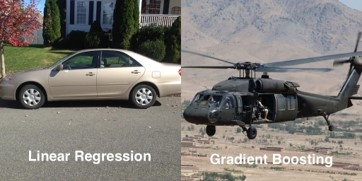
\includegraphics[width=0.95\textwidth]{pics/helicopter.jpg}
			\tiny{https://www.gormanalysis.com/blog/gradient-boosting-explained/}
		\end{figure}
	\end{columns}
\end{frame}

\begin{frame}
	\frametitle{Boosting}
	\begin{block}{Basic idea of boosting (e.g. Schapire, 1990)}
		\begin{enumerate}
			\item Fit simple model $\hat f$ to data
			\item For $k = 1, \dots, K$ do:
			\begin{itemize}
				\item[a.] Find simple model $\hat f^k$ that corrects the mistakes of $\hat f$
				\item[b.] Update: $\hat f \leftarrow \hat f + \hat f^k$
			\end{itemize}
		\end{enumerate}
	\end{block}
	
	\begin{block}{How to find updates $\hat f^k$?}
		Use decision trees $\rightarrow$ \alert{boosted trees}
		\begin{itemize}
			\item Use reweighting heuristic for binary classification
			
			$\rightarrow$ AdaBoost (Freund and Schapire, 1995)
			\item Reduce total loss $Q(\hat f + \hat f^k) = \sum_{i = 1}^n L(y_i, \hat f(\bx_i) + \hat f^k (\bx_i))$ 
			
			$\rightarrow$ \alert{Gradient boosting} (Friedman, 2001)
		\end{itemize}
	\end{block}
\end{frame}

\begin{frame}
	\frametitle{Gradient Descent}
	\begin{columns}[onlytextwidth]
		\column{0.45\textwidth}
		\begin{block}{Minimize function $h: \R^n \to \R$}
			\begin{enumerate}
				\item Start at some value $\hat x$
				\item Repeat: $\hat x \leftarrow \hat x - \lambda g$
			\end{enumerate}
			\begin{itemize}
				\item $\lambda$: Step size or learning rate
				\item Gradient of $h$ at $\hat x$:
				$$
				g = \left[\frac{\partial h(x)}{\partial x}\right]_{x = \hat x}
				$$ 
				\item $g$ points in direction of steepest ascent
			\end{itemize}
		\end{block}
		
		\column{0.55\textwidth}
		\begin{figure}
			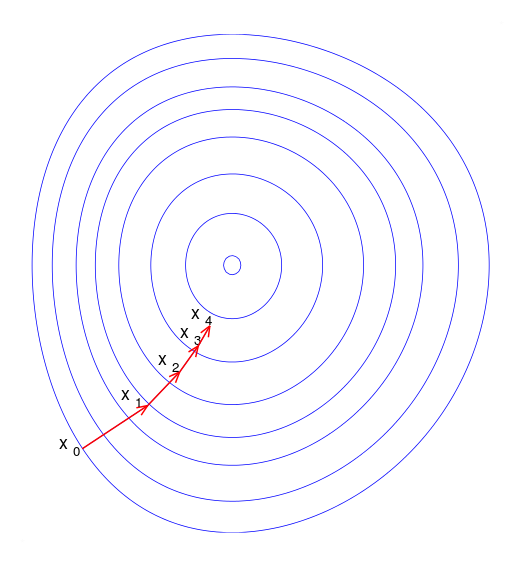
\includegraphics[width=0.8\textwidth]{../figs/gradient_descent.png}
			\tiny\url{https://en.wikipedia.org/wiki/Gradient_descent}
		\end{figure}
	\end{columns}
\end{frame}

\begin{frame}
	\frametitle{Gradient Boosting}
	\begin{columns}[onlytextwidth]
		\column{0.5\textwidth}
		\begin{block}{Gradient descent of $Q(f)$}
			\begin{itemize}
				\item $Q(f) = \sum_{i = 1}^n L(y_i, f(\bx_i))$
				\item $f = \left(f(\bx_1), \dots, f(\bx_n)\right) \in \R^n$
			\end{itemize}
			
			\begin{enumerate}
				\item Start at some value $\hat f$
				\item Repeat: $\hat f \leftarrow \hat f - \lambda g$ with
				$$
				g = \left[\frac{\partial Q(f)}{\partial f}\right]_{f = \hat f}
				$$
				having components
				$$
				g_i = \left[\frac{\partial L(y_i, f(\bx_i))}{\partial f(\bx_i)}\right]_{f(\bx_i) = \hat f(\bx_i)}
				$$
			\end{enumerate}
		\end{block}
		
		\column{0.5\textwidth}
		\begin{block}{For squared error?}
			\begin{itemize}
				\item $L(y, z) = (y-z)^2/2$
				\item Plugging in:
				$
				g_i = -(\underbrace{y_i - \hat f(\bx_i)}_{\text{Residual } r_i})
				$
				\item Repeat: $\hat f(\bx_i) \leftarrow \hat f(\bx_i) + \underbrace{\lambda r_i}_{\hat f^k \text{?}}$
			\end{itemize}
		\end{block}
		\begin{block}{Boosting with $\hat f^k = -\lambda g_i$? Now way\dots} 
			\begin{enumerate}
				\item $y_i$ unknown in application
				\item Should work for all $\bx$
			\end{enumerate}
			$\rightarrow$ replace $-g_i$ by predictions of tree
		\end{block}
	\end{columns}
\end{frame}

\begin{frame}
	\frametitle{Gradient Boosted Trees for Squared Error Loss}
	\begin{block}{Algorithm}
		\begin{enumerate}
			\item Initialize $\hat f(\bx) = \frac{1}{n}\sum_{i = 1}^{n} y_i$
			\item For $k = 1, \dots, K$ do:
			\begin{enumerate}
				\item[a.] For $i = 1, \dots, n$, calculate residuals $r_i = y_i - \hat f(\bx_i)$
				\item[b.] Model the $r_i$ as a function of the $\bx_i$ by fitting a regression tree $\hat f^k$
				\item[c.] Update: $\hat f(\bx) \leftarrow \hat f(\bx) + \lambda \hat f^k(\bx)$
			\end{enumerate}
			\item Output $\hat f(\bx)$
		\end{enumerate}
	\end{block}
	
	\begin{block}{General loss functions?}
		\begin{itemize}
			\item Replace residuals by negative gradients of loss function
			\item Leaf values might be suboptimal $\rightarrow$ replace by optimal values
		\end{itemize}
	\end{block}
\end{frame}

\begin{frame}
	\frametitle{Gradient Boosted Trees for General Losses}
	\begin{enumerate}
		\item Initialize $\hat f(\bx) = \text{argmin}_\gamma \sum_{i = 1}^{n} L(y_i, \gamma)$
		\item For $k = 1, \dots, K$ do:
		\begin{enumerate}
			\item[a.] For $i = 1, \dots, n$, calculate negative gradients (pseudo-residuals)
			$$
			r_i = -\left[\frac{\partial L(y_i, f(\bx_i))}{\partial f(\bx_i)}\right]_{f(\bx_i) = \hat f(\bx_i)}
			$$
			\item[b.] Model $r_i$ as function of $\bx_i$ by regression tree $\hat f^k$ with terminal regions $R_1, \dots, R_J$
			\item[c.] For each $j = 1, \dots, J$, use line-search to find the optimal leaf value 
			$$
			\gamma_j = \text{argmin}_{\gamma} \sum_{\bx_i \in R_j} L(y_i, \hat f(\bx_i) + \gamma)
			$$
			\vspace{-1em}
			\item[d.] Update: $\hat f(\bx) \leftarrow \hat f(\bx) + \lambda \underbrace{\sum_{j = 1}^{J} \gamma_j \boldsymbol 1\{\bx \in R_j\}}_{\text{modified tree}}$
		\end{enumerate}
		\item Output $\hat f(\boldsymbol x)$
	\end{enumerate}
\end{frame}

\begin{frame}
	\frametitle{Remarks}
	\begin{itemize}
		\item Predictions are sum of short decision trees (with modified leaf values)
		\item Random forest: average of deep trees
		\item How to select learning rate $\lambda$, number of trees $K$, \dots?
		\item (AdaBoost is gradient tree boosting with exponential loss)
	\end{itemize}
\end{frame}

\begin{frame}
	\frametitle{Modern Implementations}
	\begin{columns}[onlytextwidth]
		\column{0.5\textwidth}
		\begin{block}{Timeline}
			\begin{enumerate}
				\item XGBoost (2014)
				\item LightGBM (2016)
				\item CatBoost (2017)
			\end{enumerate}
		\end{block}
		
		\column{0.5\textwidth}
		\begin{block}{Differences to Friedman's original}
			\begin{itemize}
				\item Use of second order gradients 
				
				$\rightarrow$ no line-search necessary
				\item Histogram binning
				
				$\rightarrow$ speeds up tree growth
				
				\item Penalized objective function
			\end{itemize}
		\end{block}
	\end{columns}
	\vfill
	
	\begin{example}
	\end{example}
\end{frame}

\begin{frame}
	\frametitle{Parameter Tuning is Essential}
	\begin{columns}[onlytextwidth]
		\column{0.7\textwidth}
		\begin{enumerate}
			\item Number of boosting rounds/trees  $K$
			
			$\rightarrow$ find by early stopping (validation/CV)
			\item Learning rate $\lambda$
			
			$\rightarrow$ to get reasonable number of rounds
			\item Regularization
			\begin{itemize}
				\item Tree depth, number of leaves, loss penalties, etc.
				\item $\rightarrow$ Grid/Randomized search and iterate process
			\end{itemize}
		\end{enumerate}
		\column{0.3\textwidth}
		\begin{block}{Comments}
			\begin{itemize}
				\item Why not one big grid search on all parameters?
				\item Objective/metrics
			\end{itemize}
		\end{block}
	\end{columns}
	
	\vfill
	
	\begin{example}
		\begin{itemize}
			\item XGBoost
			\item LightGBM
		\end{itemize}
	\end{example}
\end{frame}
